 \documentclass[a4paper, 11pt]{article}
\usepackage{comment} % enables the use of multi-line comments (\ifx \fi)
\usepackage{lipsum} %This package just generates Lorem Ipsum filler text.
\usepackage{fullpage} % changes the margin
\usepackage{indentfirst}
\usepackage{graphicx}

\begin{document}
%Header-Make sure you update this information!!!!
\noindent
\large\textbf{Report: Computer Graphics} \hfill \textbf{Xucheng Chen} \\
\normalsize COMS 4160 \hfill xc2360 \\
Prof. Zheng \hfill Date: 02/23/2017

\section*{Rendered images}
    \subsection{Direct Illumination}
        \indent The direct illumination works fine for me and the resulting direct rendered image is direct-result.png and the original .xml file for it is cbox-direct.xml with sampler number of 100.
        \begin{center}
        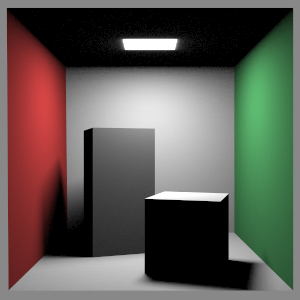
\includegraphics[width = .8\textwidth]{direct_result.PNG}
        \end{center}
    \subsection{Global Illumination}
        \indent The global illumination takes me a lot of time in debugging. Although the overall algorithm is simple and concise, the implementation involves a lot of details. The rendered image is direct-result.png and the original .xml file for it is cbox-direct.xml with sampler number of 100.
        \begin{center}
        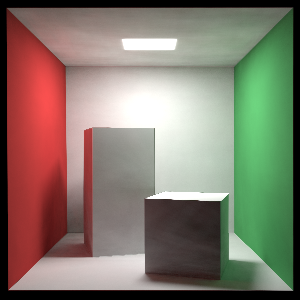
\includegraphics[width = .8\textwidth]{global_result.PNG}
        \end{center}
    \subsection{Creative Scenes}
        For the creative scene, I have set the image size to 200x200, the number of samples to 100 and the depth limit to 7 for the global illumination. If you want to change the texture type of objects, just simply change the variable texture in class Texture of package Material. The scene 1 use cbox-global-scene1.xml to render and the scene 2 use cbox-global-scene1.xml to render.
        \subsubsection{Scene1: direct illumination}
            \begin{center}
                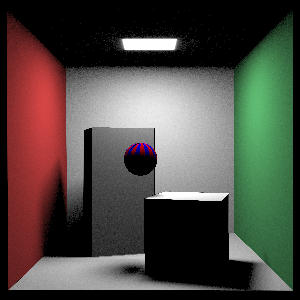
\includegraphics[width = .4\textwidth]{scene1-DI.PNG}
            \end{center}
        \subsubsection{Scene1: global illumination}
            \begin{center}
                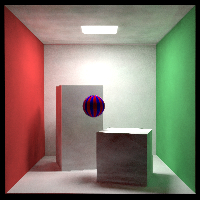
\includegraphics[width = .4\textwidth]{scene1-GI.PNG}
            \end{center}
        \subsubsection{Scene2: direct illumination}
            \begin{center}
                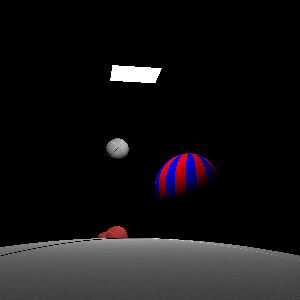
\includegraphics[width = .4\textwidth]{scene2-DI.PNG}
            \end{center}
            Below is the direct illumination image of scene 2 using image texture, which takes very long time to render.
            \begin{center}
                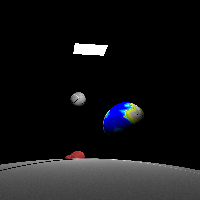
\includegraphics[width = .4\textwidth]{scene2-DI-IMAGE.PNG}
            \end{center}
        \subsubsection{Scene2: global illumination}
            \begin{center}
                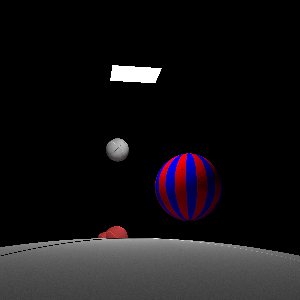
\includegraphics[width = .4\textwidth]{scene2-GI.PNG}
            \end{center}
%Put your Problem statement here! Example of a Citation\cite[p.219]{Robotics}. Here's Another Citation\cite{Flueck}

\section*{External resources}
    \indent There are some packages called libnoiseforjava, which is the java wrapper of libnoise on github. I used these packages to generate the image texture picture, which is called noise.png.

\section*{Bonus extension}
    \indent As I mentioned earlier, I have successfully map the texture on objects by creating a Material class named Texture.java, but it only works for spheres. The result is shown in "cbox-direct-image-texture.png".

\section*{Reminder}
   \indent If you try to do image-texture rendering, you should wait about half an hour, while the others are quite faster. I strongly recommend using procedural texture instead.
\ifx

\section*{Analysis \& Testing}
\lipsum[6]

\section*{Final Evaluation}
\lipsum[7]

\section*{Attachments}
%Make sure to change these
Lab Notes, HelloWorld.ic, FooBar.ic
%\fi %comment me out

\begin{thebibliography}{9}
\bibitem{Robotics} Fred G. Martin \emph{Robotics Explorations: A Hands-On Introduction to Engineering}. New Jersey: Prentice Hall.
\bibitem{Flueck}  Flueck, Alexander J. 2005. \emph{ECE 100}[online]. Chicago: Illinois Institute of Technology, Electrical and Computer Engineering Department, 2005 [cited 30
August 2005]. Available from World Wide Web: (http://www.ece.iit.edu/~flueck/ece100).
\end{thebibliography}
\fi
\end{document} 